\def\difficulty{1}
\sujet{Integral Geometry}
\index{Geometry!Integral Geometry}

\label{tutorial:integral_geometry:enonce}

\begin{note}This tutorial aims to characterize objects by measurements from integral geometry.
\end{note}


The different processes will be applied on the following synthetic image:
\vspace*{-5pt}
\begin{figure}[H]
\centering

\includegraphics[height=3.5cm]{X.png}
\caption{$X$}
\label{fig:integral_geometry:enonce:X}
\end{figure}

\vspace*{-10pt}

\section{Cell configuration}
\vspace*{-5pt}
\index{Topology!Neighborhood}
\textls[-15]{The spatial support of an image can be covered by cells associated with pixels. A cell (square of interpixel distance size) is composed of 1 face, 4 edges and 4 vertices. Either a cell is centered in a pixel (intrapixel cell) or a cell is constructed by connecting pixels (interpixel cell). The following figure shows the two possible representations of an image with 16 pixels:}
\vspace*{-10pt}
\begin{figure}[H]
\centering\caption{Pixels representation.}
\subfloat[Image.]{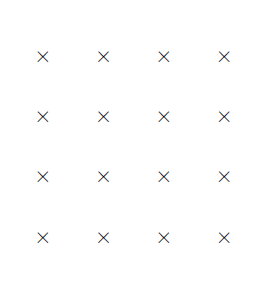
\includegraphics[height=4cm]{cell1.png}}\hfill
\subfloat[Intrapixel cells.]{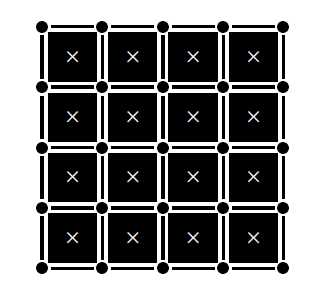
\includegraphics[height=4cm]{cell2.png}}\hfill
\subfloat[Interpixel cells.]{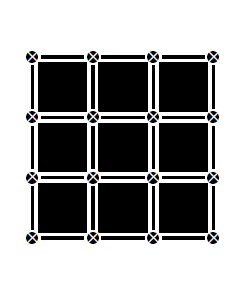
\includegraphics[height=4cm]{cell3.png}}%
\label{fig:integral_geometry:enonce:configurations}\vspace*{-10pt}%
\end{figure}
\vspace*{-5pt}

We respectively denote $f^{intra}$ (resp. $f^{inter}$), $e^{intra}$ (resp. $e^{inter}$) and $v^{intra}$ (resp. $v^{inter}$) the number of faces, edges and vertices for the intrapixel (resp. interpixel) cell configuration
Using these two configurations, the measurements from integral geometry (area $A$, perimeter $P$, Euler number $\chi_8$ or $\chi_4$) can be computed as:\vspace*{-5pt}
\begin{eqnarray}
A&=&f^{intra}=v^{inter}\label{eq:integral_geometry:aire}\\
P&=&-4f^{intra}+2e^{intra}\\
\chi_8&=&v^{intra}-e^{intra}+f^{intra}\\
\chi_4&=&v^{inter}-e^{inter}+f^{inter}\label{eq:integral_geometry:euler4}
\end{eqnarray}

\begin{qbox}
\begin{enumerate}
	\item Count manually the number of faces, edges and vertices of the image $X$ for the two configurations (Intra- and Inter-pixel) of Fig. \ref{fig:integral_geometry:enonce:X}.
	\item Deduce the measurements from integral geometry (Eq. \ref{eq:integral_geometry:aire}-\ref{eq:integral_geometry:euler4}).
\end{enumerate}	
\end{qbox}
\vspace*{-5pt}
\section{Neighborhood configuration}\vspace*{-5pt}
In order to efficiently calculate the number of vertices, edges and faces of the object, the various neighborhood configurations (of size 2x2 pixels) of the original binary image $X$ are firstly determined. Each pixel corresponds to a neighborhood configuration $\alpha$. Thus, sixteen configurations are possible, presented in Tab. \ref{tab:integral_geometry:enonce:neighborhoods}.

\vspace*{-8pt}
\begin{table}[H]
\caption{Neighborhood configurations.}%
\centering
\begin{tabular}{|l|ll|ll|ll|ll|ll|ll|ll|ll|}
\hline
 & 0 & 0 & 0 & 0 & 0 & 1 & 0 & 1 & 0 & 0 & 0 & 0 & 0 & 1 & 0 & 1\\
 & 0 & 0 & 0 & 1 & 0 & 0 & 0 & 1 & 1 & 0 & 1 & 1 & 1 & 0 & 1 & 1\\ \hline
$\alpha$ & \multicolumn{2}{c|}{0} & \multicolumn{2}{c|}{1} & \multicolumn{2}{c|}{2} & \multicolumn{2}{c|}{3} & \multicolumn{2}{c|}{4} & \multicolumn{2}{c|}{5} & \multicolumn{2}{c|}{6} & \multicolumn{2}{c|}{7}\\ \hline\hline
 & 1 & 0 & 1 & 0 & 1 & 1 & 1 & 1 & 1 & 0 & 1 & 0 & 1 & 1 & 1 & 1\\
 & 0 & 0 & 0 & 1 & 0 & 0 & 0 & 1 & 1 & 0 & 1 & 1 & 1 & 0 & 1 & 1\\ \hline
$\alpha$ & \multicolumn{2}{c|}{8} & \multicolumn{2}{c|}{9} & \multicolumn{2}{c|}{10} & \multicolumn{2}{c|}{11} & \multicolumn{2}{c|}{12} & \multicolumn{2}{c|}{13} & \multicolumn{2}{c|}{14} & \multicolumn{2}{c|}{15} \\
\hline
\end{tabular}
\label{tab:integral_geometry:enonce:neighborhoods}%\vspace*{-10pt}
\end{table}
\vspace*{-8pt}

Thereafter, each configuration contributes to a known number of vertices, edges and faces (Tab. \ref{tab:integral_geometry:enonce:contributions}). To determine the neighborhood configurations of all the pixels, an efficient algorithm effective consists in convolving the image $X$ by a mask $F$, whose values are powers of two, and whose origin is the top-left pixel:\vspace*{-5pt}
$$
F=\left(
\begin{array}{cc}
1 & 4\\
2 & 8
\end{array}
\right)
$$
\textls[-5]{The resulting image is $X*F$. Notice that this image $X$ has no pixel touching the borders, your code should ensure this (for example by padding the array with zeros).
In this way, the histogram $h$ of $X*F$ gives the distribution of the neighborhood configurations from image $X$. And each configuration contributes to a known number of vertices, edges and faces:}\vspace*{-5pt}
\begin{eqnarray}
v&=&\sum_{\alpha=0}^{15}v_{\alpha}h(\alpha)\\
e&=&\sum_{\alpha=0}^{15}e_{\alpha}h(\alpha)\\
f&=&\sum_{\alpha=0}^{15}f_{\alpha}h(\alpha)
\end{eqnarray}

The following table gives the values of $v_{\alpha}$, $e_{\alpha}$ and $f_{\alpha}$ for each cell configuration.

\begin{qbox}
	\begin{enumerate}
		\item Compute the distribution of the neighborhood configurations from image $X$.
		\item Deduce the number of vertices, edges and faces for each cell representation and compare these values with the previous (manually computed) results.
	\end{enumerate}
\end{qbox}

\begin{table}[H]
\centering\caption{\textls[-20]{Contributions of the neighborhood configurations to the computation of $v, e$ and $f$}}
\begin{tabular}{|c|c|c|c|c|c|c|c|c|c|c|c|c|c|c|c|c|}
\hline
\multicolumn{17}{|c|}{intrapixel cells}\\\hline
$\alpha$&0&1&2&3&4&5&6&7&8&9&10&11&12&13&14&15\\\hline
$f_{\alpha}$&0&1&0&1&0&1&0&1&0&1&0&1&0&1&0&1\\\hline
$e_{\alpha}$&0&2&1&2&1&2&2&2&0&2&1&2&1&2&2&2\\\hline
$v_{\alpha}$&0&1&1&1&1&1&1&1&1&1&1&1&1&1&1&1\\\hline\hline
\multicolumn{17}{|c|}{interpixel cells}\\\hline
$\alpha$&0&1&2&3&4&5&6&7&8&9&10&11&12&13&14&15\\\hline
$f_{\alpha}$&0&0&0&0&0&0&0&0&0&0&0&0&0&0&0&1\\\hline
$e_{\alpha}$&0&0&0&1&0&1&0&2&0&0&0&1&0&1&0&2\\\hline
$v_{\alpha}$&0&1&0&1&0&1&0&1&0&1&0&1&0&1&0&1\\\hline
\end{tabular}
\label{tab:integral_geometry:enonce:contributions}
\end{table}

\vspace*{-10pt}
\section{Crofton perimeter}\vspace*{-5pt}
\index{Geometry!Crofton Perimeter}
The Crofton perimeter could be computed form the number of intercepts in different random directions. In discrete case, only the directions $0, \pi/4, \pi/2$ and $3\pi/4$ are considered; they are selected according to the desired connexity.

The number of intercepts are denoted $i_0, i_{\pi/4}, i_{\pi/2}$ and $i_{3\pi/4}$ for the orientation angles $0, \pi/4, \pi/2$ and $3\pi/4$ respectively.

In this way, the Crofton perimeter (in 4 and 8 connexity) is defined in discrete case as:
\begin{eqnarray}
P_4&=&\frac{\pi}{2}\left(i_0+i_{\pi/2}\right)\\
P_8&=&\frac{\pi}{4}\left(i_0+\frac{i_{\pi/4}}{\sqrt{2}}+i_{\pi/2}+\frac{i_{3\pi/4}}{\sqrt{2}}\right)
\end{eqnarray}
These perimeter measurements can be computed from the neighborhood configurations of the original image:\vspace*{-15pt}
\begin{eqnarray}
P_4&=&\sum_{\alpha=0}^{15}P^4_{\alpha}h(\alpha)\\
P_8&=&\sum_{\alpha=0}^{15}P^8_{\alpha}h(\alpha)
\end{eqnarray}
with the following weights $P^4_{\alpha}$ and $P^8_{\alpha}$ of these linear combinations (Tab. \ref{tab:integral_geometry:enonce:crofton}):

\begin{table}[H]
\centering\caption{Weights for the computation of the Crofton perimeter}%
$\begin{array}{|c|c|c|c|c|c|c|c|c|}
\hline
\alpha&0&1&2&3&4&5&6&7\\\hline
P^4_{\alpha}&0&\frac{\pi}{2}&0&0&0&\frac{\pi}{2}&0&0\\\hline
P^8_{\alpha}&0&\frac{\pi}{4}\left(1+\frac{1}{\sqrt{2}}\right)&\frac{\pi}{4\sqrt{2}}&\frac{\pi}{2\sqrt{2}}&0&\frac{\pi}{4}\left(1+\frac{1}{\sqrt{2}}\right)&0&\frac{\pi}{4\sqrt{2}}\\
\hline
\hline
\alpha&8&9&10&11&12&13&14&15 \\ \hline
P^4_{\alpha}&\frac{\pi}{2}&\pi&0&0&\frac{\pi}{2}&\pi&0&0 \\ \hline
P^8_{\alpha}&\frac{\pi}{4}&\frac{\pi}{2}&\frac{\pi}{4\sqrt{2}}&\frac{\pi}{4\sqrt{2}}&\frac{\pi}{4}&\frac{\pi}{2}&0&0 \\
\hline
\end{array}$
\label{tab:integral_geometry:enonce:crofton}
\end{table}

\begin{qbox}
 Evaluate the perimeters $P_4$ and $P_8$ with the previous formula on Fig.\ref{fig:integral_geometry:enonce:X}
\end{qbox}
